% !TEX program = XeLaTeX
% !TEX encoding = UTF-8
\documentclass[UTF8,nofonts]{ctexart}
\setCJKmainfont[BoldFont=FandolSong-Bold.otf,ItalicFont=FandolKai-Regular.otf]{FandolSong-Regular.otf}
\setCJKsansfont[BoldFont=FandolHei-Bold.otf]{FandolHei-Regular.otf}
\setCJKmonofont{FandolFang-Regular.otf}

\usepackage{url}
\usepackage{cancel}
\usepackage{xspace}
\usepackage{graphicx}
\usepackage{multicol}
\usepackage{multirow}
\usepackage{subfig}
\usepackage{amsmath}
\usepackage{amssymb}
%\usepackage[a4paper,width=180mm,top=18mm,bottom=22mm,includeheadfoot]{geometry}
\usepackage[a4paper,width=140mm,top=18mm,bottom=22mm,includeheadfoot]{geometry}
\usepackage{booktabs}
\usepackage{array}
\usepackage{verbatim}
\usepackage{caption}
%\usepackage{natbib}
\usepackage{booktabs}
\usepackage{float}
\usepackage{pdflscape}
%\usepackage{draftwatermark}
\usepackage{mathtools}
\usepackage[usenames,dvipsnames]{xcolor}
\usepackage{afterpage}
\usepackage{pgf}
\usepackage{tikz}
\usepackage{dirtree}
\usepackage{amsfonts}
\usepackage{tkz-graph}
\newtheorem{definition}{定义}[section]
\newtheorem{theorem}{定理}[section]
\newtheorem{lemma}{Lemma}
\newtheorem{proof}{证明} [section]
\usepackage[toc,page,title,titletoc,header]{appendix} 
\renewcommand\appendixname{目\ 录}
\renewcommand\appendixpagename{附\ 录}
\usetikzlibrary{shapes.geometric}%

%\SetWatermarkText{请勿传播}
%\SetWatermarkColor[rgb]{1,0,0}
%\SetWatermarkScale{0.2}


\title{Multilateral Token Exchange (MTX) Protocol\\一个以太坊代币的多边交易协议\\(草稿 v0.1)}
\author{ 
    dong77@gmail.com\\
%    \and
    fdwanghui@gmail.com    % lihaomin@zhongan.io
}

\makeatletter
\def\CTEX@section@format{\Large\bfseries}
\makeatother

\makeatletter
\newenvironment{tablehere}
  {\def\@captype{table}}
  {}

\newenvironment{figurehere}
  {\def\@captype{figure}}
  {}
\makeatother


\begin{document}
\maketitle

\begin{abstract}
本文描述一个开放的,以太坊上ERC20代币间的多边交易协议。通过该协议,可以建立去中心化且无需资产托管的交易所应用。该协议可被视为下一代数字资产交易所的开放标准之一和架构基石。传统交易所可以通过拥抱该协议改进目前交易所的撮合方式,降低用户信任成本和自身运营风险;去中心化应用(dApp)也可也以在智能合约中调用该协议的相关智能合约实现应用内的代币转换。

\end{abstract}

\newpage

\tableofcontents
\newpage

\section{背景\label{sec:background}}

区块链作为比特币的底层技术,本质上是去中心化无信任环境中的存在性共识。存在性可应用于各种不同的数据,如股权,版权,使用权等。尽管联盟链和企业私有链中共识数据的类别正在变得越来越多样化,但这些数据的价值却有着明确的边界限制 - 只限于联盟成员间和企业内部。我们认为区块链的价值网络属性在公有链中才会的到更好的体现。根据coinmarketcap.com的统计,截止本文成稿时间,区块链上代币总市值已经超过790亿美元,以太坊区块链上承载的代币市值超过170亿美元。

区块链对各个行业都将有着深远的影响,尤其是金融领域。我们相信基于区块链的新金融会有一个明显趋势,即资产代币化(Tokenization):一方面链下资产的使用权,所有权,分红权等相关权益产通过抵押会被发行到区块链上,另一方面区块链上资产也会进行跨链发行。资产代币化的重要目标之一就是低成本,全球化,全天候的高流动性,而流动性则主要通过交易机制和交易所得以实现。

在现阶段,提供主要流动性的交易所都有非常类似的模式:交易所要求用户将法币或者代币充值到交易所的银行或区块链账户中,然后交易所在自己中心服务器的虚拟账户系统中为用户进行IOU记账。用户实际交易的是这些IOU。为了将IOU兑换成法币或区块链代币,用户需要向交易所提出提现请求,提现成功后,才算真正交易完成。在这个过程中,交易所替用户安全保管资产的能力是用户最大的风险;同时用户还需担心交易所运营者的商业道德问题,比如挪用资金造成资不抵债等。2014年2月当时世界最大规模的比特币交易所运营商Mt.Gox的85万个比特币被盗一空,公司向日本东京地方法院申请破产保护。该公司的用户至今仍在等待其返还尚未被盗的少量比特币。随着调查的不断进行Mt.Gox被曝出所谓的比特币被盗其实是监守自盗。85万个“被偷窃”的比特币中,实际上因外部盗窃失踪的仅为7000个。2016年8月最大的美元比特币交易平台香港的Bitfinex由于网站出现安全漏洞,导致用户持有的比特币被盗,被盗的比特币共119756枚,总价值约为6500万美元。随后该公司决定由所有用户共同分担损失以避免其破产。交易所缺失的资产保管能力和监守自盗的败坏的商业道德,一方面反映出比特币在各个国家监管政策的缺失与漏洞,另一方面也证实中心化交易所模式的固有风险。

基于区块链的去中心化交易机制就是为了彻底解决上述问题。去中心化交易的核心优势之一是避免任何资产被托管,因此资产就不存在被盗的可能性,这会极大降低用户对交易所的信任成本;这种交易机制的另一个优势是没有地缘和时间限制,以及极高的透明性和可追溯性。这些特点会促使交易整体具有更大的流动性和更小的买卖价差。

\section{相关工作\label{sec:existingworks}}

开源社区已经有过一些基于区块链搭建去中心化的交易所的尝试,如瑞波(Ripple)、比特股(BitShares)、Openledger等。
Ripple \cite{schwartz2014ripple} 是一个去中心化的银行系统间清算协议,是为了解决银行间清算的高费用和高延迟问题而设计,具有快速、方便、超低费用的优点。Ripple提出了一项Interledger \cite{thomas2015protocol} 协议(ILP)实现跨账本的资产交易。ILP 本身并不是一个账本,相反,它提供了一个顶层加密托管系统,在称之为“连接者”的中介机构的帮助下,可以让资金在各账本之间进行流动。

比特股 \cite{schuhbitshares}\cite{schuh2015bitshares}  是一个基于区块链的开发平台,任何个人和机构都可以在此平台上自由地进行转账、借贷、发行资产等,也可以基于这个平台快速搭建出去中心化的金融服务平台等。BitShares 内置的去中心化交易所(DEX),让数字资产的交易撮合和交割完全发生在链上,并通过内置智能合约锚定其他资产,如法币、比特币、黄金、白银等。

Openledger是一个新型去中心化交易平台。它允许用户将比特币兑换成法币锚定的 SmartCoins,SmartCoins 可以直接通过 paypal、 瑞波网关以及 CCEDK 的 NanoCard 兑换成现金。需要注意的是,Openledger在很大程度上依赖于比特股 2.0平台以及 Cryptonomex 开发的 Graphene Toolkit。因此,Openledger平台的性能取决于Graphene Toolkit的性能和比特股 2.0平台的性能。

比特币的闪电网络和以太坊上的雷霆网络\cite{poon2015bitcoin}是一个去中心化的系统。它们的卓越之处在于,无需信任对方以及第三方即可实现实时的、海量的交易网络。闪电网络和雷霆网络提供了一个可扩展的微支付通道网络。交易双方若在区块链上预先设有支付通道,就可以多次、高频、双向地通过轧差方式实现瞬间确认的微支付;双方若无直接的点对点支付通道,只要网络中存在一条连通双方的、由多个支付通道构成的支付路径,闪电网络和雷霆网络也可以利用这条支付路径实现资金在双方之间的可靠转移。


Bancor协议引入了一种基于数学模型的方案去试图解决经济学中的“双重需求巧合”问题,理念和预测市场中的Logarithmic Market Scoring Rules(LSMR)类似。它声称使用以区块链为基础的智能合约和储备货币,可以允许任何人通过这个协议创建代币,代币以预先设置的比率来持有一种或几种其它代币作为自己的储备金。这些储备代币可以是法币、数字化资产或其它加密货币。通过使用这些储备金,不论有没有交易,新创建的代币都可以获得价值。此外,不论有没有买家,这些新创建的代币都可以随时兑换回其储备代币。

0x \cite{warren20170x} 是一个可以在以太坊区块链上进行 ERC20 代币对等交易的开放式协议。该协议旨在成为通用开放标准,作为可与其他协议组合的基本模块,用以驱动越来越复杂的区块链应用程序。由于它使用的是公开访问的智能合约系统,因此可以作为各种 dApps 的共享基础架构。而从长远来看,开放式技术标准相比封闭模式具有更大的优势,随着每个月有更多的资产在区块链上被代币化,也有更多的 dApps 需要使用这些不同的代币,开放式标准也因此变得更加重要。此外,由 dApps 耦合到其底层协议所导致的智能合约冗余也是未来区块链协议开发的主要障碍,因此在标准化之余,我们还需要一个合适的解耦方式。0x 协议试图将信息交换功能从应用层拉到协议层,推动 dApps 之间的互操作性。然而,0x协议具有以下局限性:taker必须在线匹配订单,这导致撮合实时性差,难以优化成交价格;0x协议采用的是简单的OTC方式,无法法实现复杂订单的撮合;不同交易所之间没有明确的竞争激励机制;没有考虑了矿工的利益。

然后上述努力由于种种限制,到目前为止依然没有能够撼动中心化交易所的地位。我们受到支付通道和0x协议的启发,提出一种可行的,基于区块链技术的交易撮合标准。


\section{协议设计\label{sec:protocol}}

\begin{center}
\begin{figurehere}
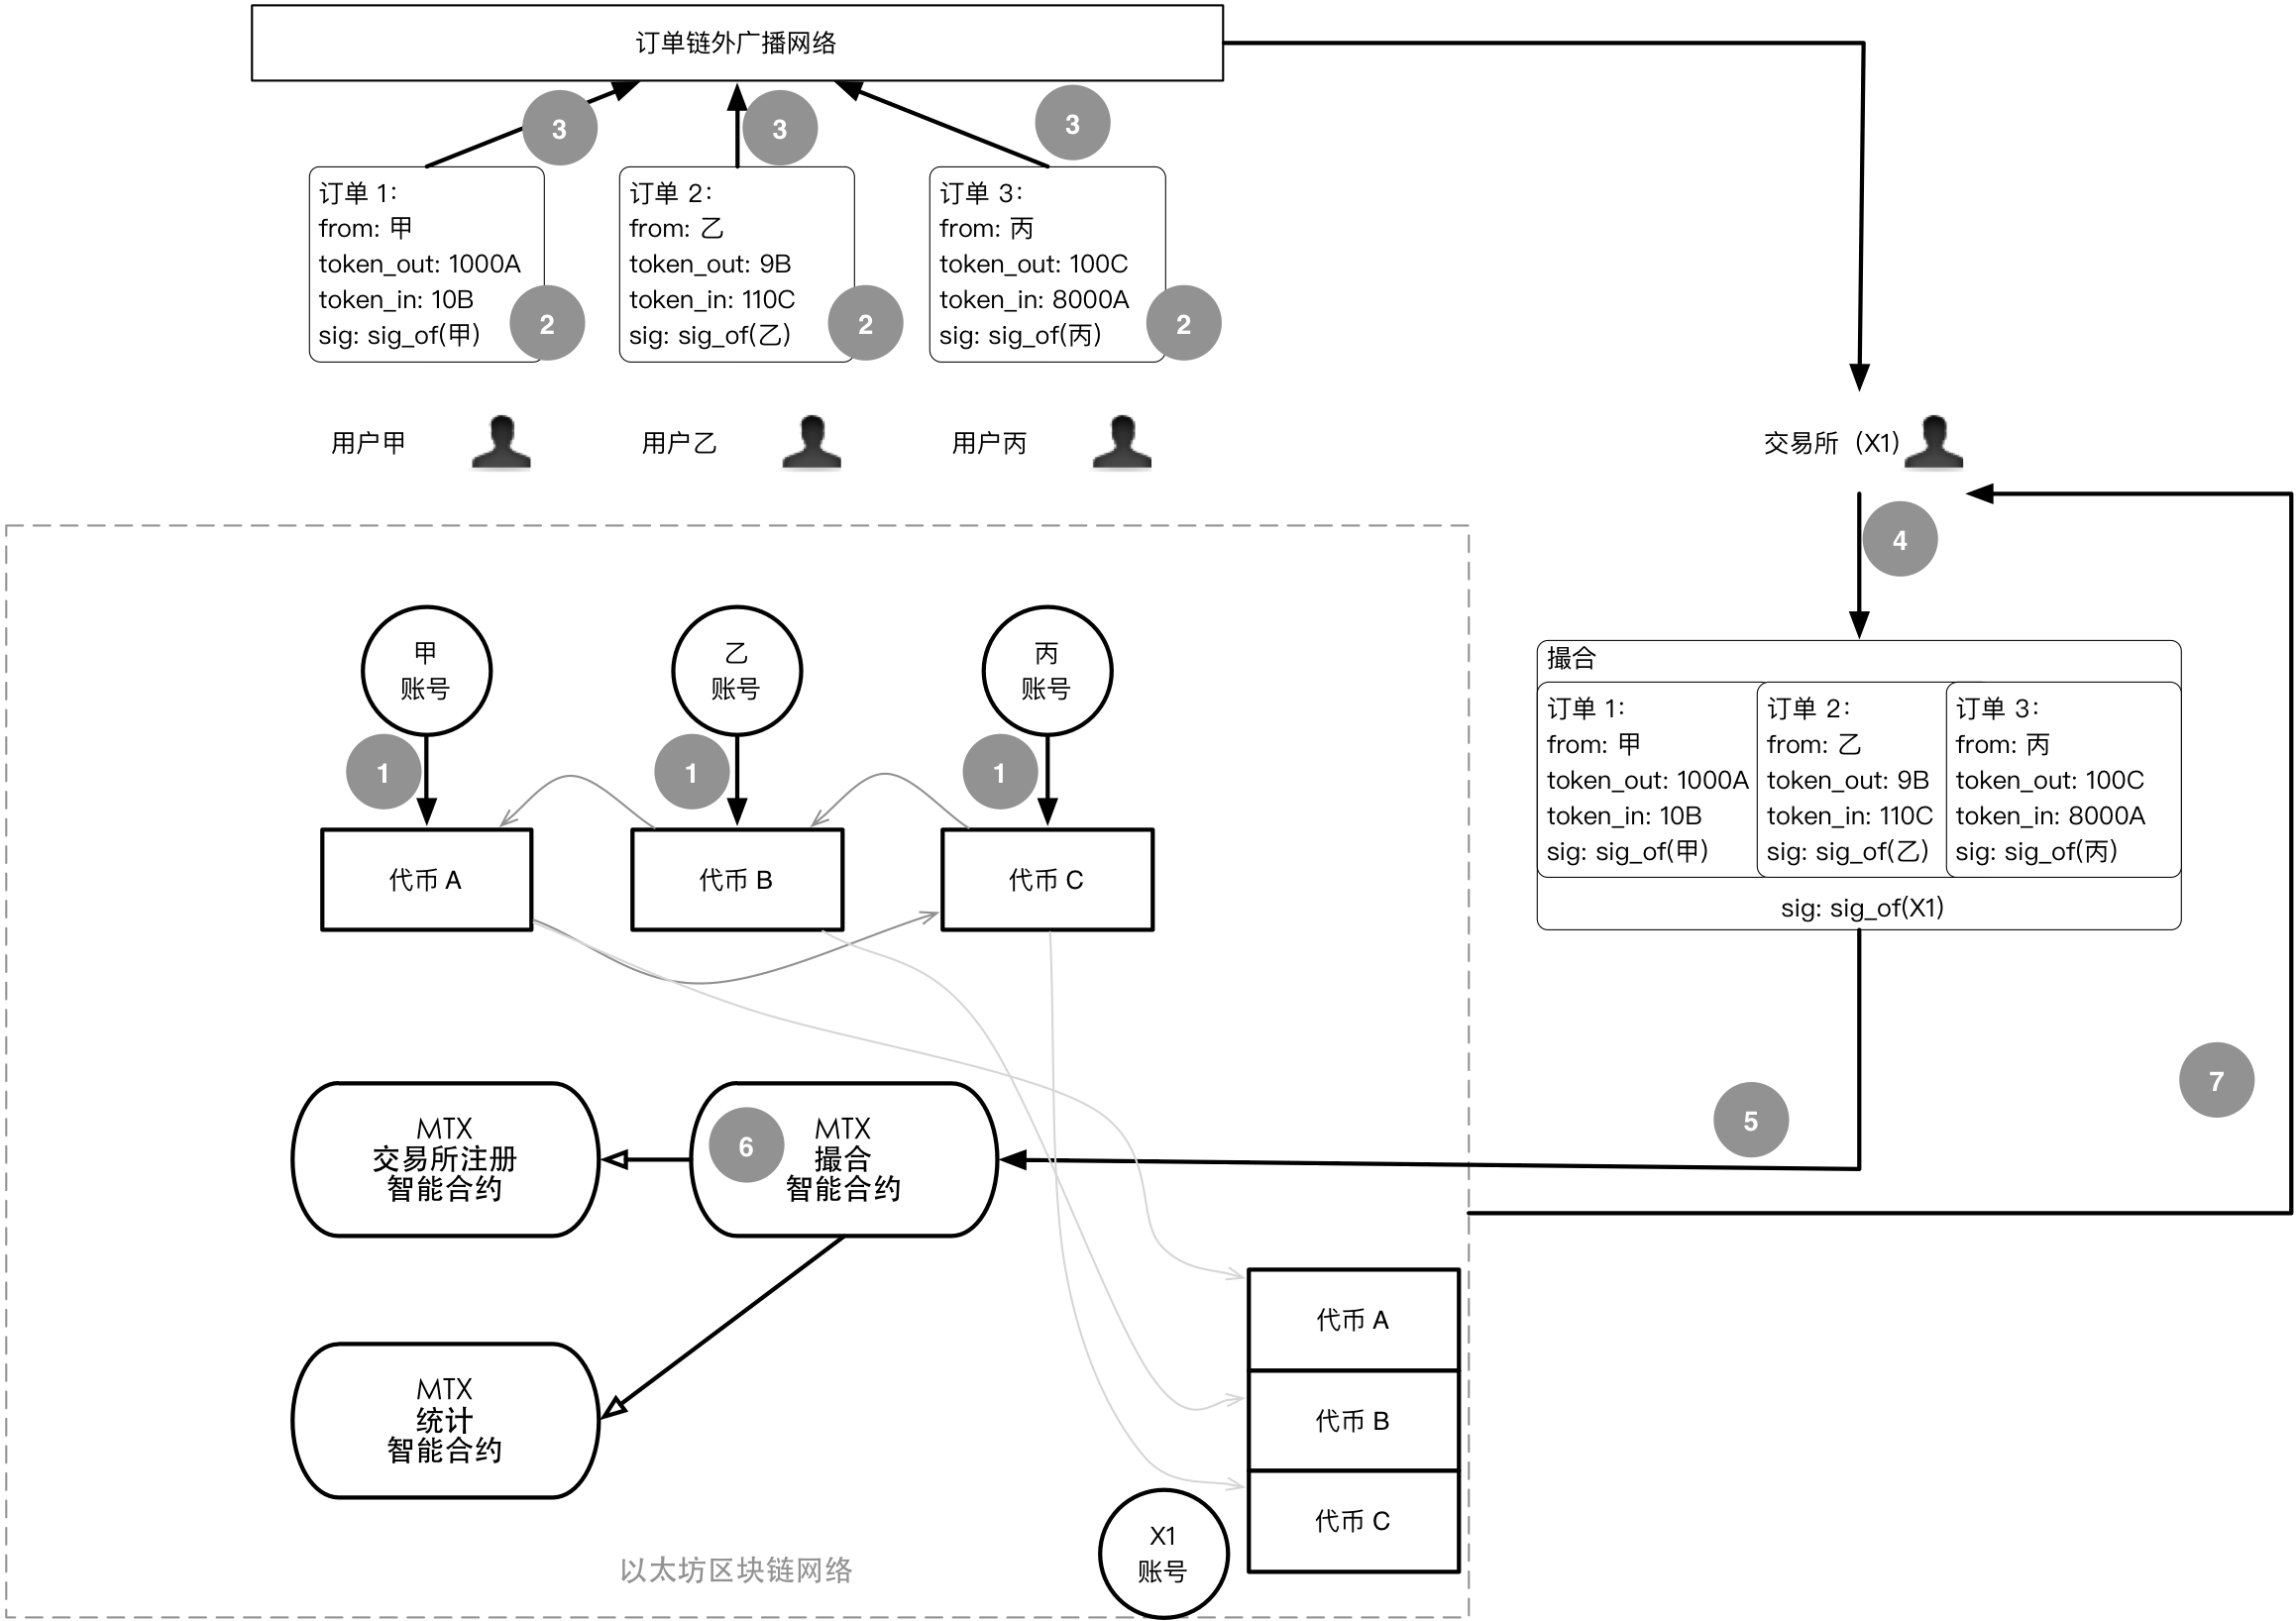
\includegraphics[height=10cm]{images/mtx-protocol.png}
\caption{MTX协议:图中示例一个三边交易的撮合}
\label{fig:mtxprotocol}
\end{figurehere}
\end{center}

我们用上图中的三边交易,简要讲解下采用MTX协议的撮合交易过程。该过程如下:

\begin{enumerate}
	\item 用户甲、乙、丙分别对MTX撮合智能合约(MTX Matching Contract)授权,授权后该合约可对用户指定代币账号做不超过一定额度的转出操作。在上面实例中,合约可最多从用户甲的账号转出1000个$A$代币,从用户乙账户转出9个$B$代币,从用户丙账户转出100个$C$代币;
	\item 用户甲、乙、丙分别生成自己的订单,并用私钥对其进行数字签名。订单的表示不再区分买单和卖单,所有订单都被视为\texttt{交换单} --- 甲的订单声明:甲愿意卖出不多于1000个$A$代币,买到尽可能多但不少于10个$B$代币;如果是部分成交,那么$A$到$B$的\texttt{兑换率}不得低于1000/10 = 100.0(卖出代币数量除以买入代币数量)。订单中还可以包含其它参数,我们在章节\ref{sec:dataformat}中会进一步说明这些参数;
	\item 甲、乙、丙分别将自己的订单通过适当的方式发送到一个或多个交易所;
	\item 交易所收到上述三个订单,将它们分别放到三个对应的订单表(orderbook)中,并实时通过区块链数据更新计算每个订单的状态,同时不断努力寻找能够撮合的一组订单 --- 我们后续称之为\texttt{交易环路}或者\texttt{撮合环路}。一旦确定三个订单的当前状态可以撮合成功,且收益(交易手续费加分润减去以太坊gas消耗)满足预期,即决定实施这个撮合;
	\item 交易所对撮合交易签名后发送到以太坊上的MTX撮合智能合约地址;
	\item 撮合智能合约验证四方签名,之后验证三个订单(的最新状态)是否可以真正成交。若无法成交,合约终止;否则智能合约分别计算出甲、乙、丙三方各自需要支出的金额,以及交易所该收取的费用,并且实时将甲、乙、丙账号中的资产进行互转,并完成对交易所的费用支付。在交易过程中,撮合智能合约还会调用MTX注册智能合约(MTX Registration Contract)来计算交易所应该给予该笔交易的费用折扣;在交易完成前,还会调用MTX统计智能合约(MTX Stats Contract)对交易所以及代币相关的统计数据做更新。
	\item 交易所监听新的区块和链下新的交易数据,并根据这些数据更新订单表,然后不断进行新的撮合。
\end{enumerate}

在传统交易所模型中,被撮合的两方中先下单的为Maker,后下单的为Taker。因为Maker创造流动性而Taker销毁流动性,所以在计算成交价时候会更偏向于Maker的价格,甚至直接采用Maker的价格作为成交价。与之相比,MTX采用的是Over-The-Counter(OTC)模型。主要的原因是在去中心化环境中,很难严格界定哪个单是真正意义上较早的单。因此MTX的撮合设计不考虑时间因素,只考虑兑换率(在本文中我们偶尔也用价格一词与兑换率交替使用)。

MTX协议的另一个显著特点是消除了传统交易所中\texttt{交易对(Trading Pair)}的概念。一个从$A$到$B$的订单不一定要一个反向的从$B$到$A$订单才能撮合,只要有一个交易环路被发现,就可以撮合。也可以说传统交易所的交易对是多边交易环路的一个最简特例。

接下来我们介绍可以撮合成交的交易环路相关的概念,包括\texttt{交易链},交易链的可归约性,成交价,成交量,和交易所收益模型。

\subsection{符号定义}

在正式介绍协议之前,我们要介绍一些符号的定义。
\[
\begin{split}
&C_{i}\text{ :}\text{编号为$i$的代币币种。}\\
&O_{i\rightarrow j}\text{:}\text{一个卖出代币为$C_{i}$,买入代币为$C_{j}$的订单。}\\
&s_{i\rightarrow j}\text{:}\text{表示上述订单的当前卖出代币$C_{i}$的数量。}\\
&b_{i\rightarrow j}\text{:}\text{表示上述订单的当前买入代币$C_{j}$的数量。}\\
&r_{i\rightarrow j}\text{:}\text{为订单$O_{C_{i}\rightarrow C_{j}}$的兑换率,即$s_{i\rightarrow j}/b_{i\rightarrow j}$}。
%&t^{a}_{i\rightarrow j}\text{:}\text{表示上述订单中MTX代币的数量,用于撮合费用。}\\
%&\beta^{a}_{i\rightarrow j}\text{:}\text{表示上述订单中的成交价分润比例。}\\
。
\end{split}
\]


为了特指订单的原始状态,我们为符号加上水平线,代表其在原始订单中的值,比如$\overline{s}_{i\rightarrow j}$和$\overline{b}_{i\rightarrow j}$本别代表原始订单中的卖出和买入货币数量。

\subsection{订单兑换率恒定\label{sec:consistrate}}

除非订单完全成交,即$s_{i\rightarrow j} == 0$,否则MTX协议保证订单状态更新后:
$s_{i\rightarrow j}/b_{i\rightarrow j} == \overline{s}_{i\rightarrow j}/\overline{b}_{i\rightarrow j}$,即订单中隐含的兑换率不会因为部分成交而变化,亦即$r_{i\rightarrow j} == \overline{r}_{i\rightarrow j}$

\subsection{可规约性\label{sec:reducability}}


考虑两个订单$O_{i\rightarrow j}$和$O_{j\rightarrow k}$,我们可以通过中间代币$C_j$的连接,将其规约一个卖出代币为$Ci$,买入代币为$C_k$的订单。我们用$O_{i\rightarrow j\rightarrow k}$来表示这样一个订单,它和订单$O_{i\rightarrow k}$在撮合的各种属性上是等价的,且:

\begin{equation}
s_{i\rightarrow j\rightarrow k}=min(b_{i\rightarrow j},s_{j\rightarrow k}) \cdot r_{i\rightarrow j}
\end{equation}

\begin{equation}
b_{i\rightarrow j\rightarrow k}=min(b_{i\rightarrow j},s_{j\rightarrow k}) \div r_{j\rightarrow k}
\end{equation}

\begin{equation}
r_{i\rightarrow j\rightarrow k}= r_{i\rightarrow j}\cdot r_{j\rightarrow k}
\end{equation}


在这里我们顺便引入\texttt{订单链}这个概念。一个订单链是两个或者两个以上订单,除了最后一个订单,每个订单的买入代币类型恰巧是后一个订单的卖出代币类型,但最后一个订单的买入代币类型不同于第一个订单的卖出代币类型(否则就成了一个环路)。我们可以将上述规约计算用于一个订单链。通过规约,一个包含$n-1$个订单($n$个不同的代币),即长度为$n-1$的订单链可被视为一个单一订单$O_{0\rightarrow ...\rightarrow n}$,且有:

\[ s_{0\rightarrow ...\rightarrow n} =
  \begin{cases}
    s_{0\rightarrow 1}      & \quad \text{如 } n \text{ == 1}\\
    min(b_{0\rightarrow ...\rightarrow n-1},s_{n-1\rightarrow n}) \cdot r_{0\rightarrow ...\rightarrow n-1}  & \quad \text{如} n \text{ > 1}\\
  \end{cases}
\]

\[ b_{0\rightarrow ...\rightarrow n} =
  \begin{cases}
    b_{0\rightarrow 1}      & \quad \text{如 } n \text{ == 1}\\
    min(b_{0\rightarrow ...\rightarrow n-1},s_{n-1\rightarrow n}) \div r_{n-1\rightarrow n}  & \quad \text{如} n \text{ > 1}\\
  \end{cases}
\]


\[ r_{0\rightarrow ...\rightarrow n} = \prod_{i=0}^{n-1}{r_{i\rightarrow i+1}}
\]


订单链的可规约性可以帮助我们在分析订单路径时简化模型,在后文的讨论中,我们将符号$O_{i \rightarrow j}$的含义扩展到即包含简单的卖出代币为$C_i$,买入代币为$C_j$的单一订单,也包含可规约成这样一个类型订单的订单链,如果为了强调是个订单链,我们会用$O_{i \rightarrow ...\rightarrow j}$或$O_{i \rightarrow \rightarrow j}$表示。

\subsection{环路撮合}

传统撮合系统是在两个币种间,即一个交易对的买卖两个方向间完成撮合;而MTX协议将撮合的概念扩展到多币种,通过\texttt{交易环路}来完成多个币种之间交易的撮合。下面介绍一下交易环路的概念。

\begin{definition}[交易环路]
假定有$n$个币种$C_{0}$、$C_{1}$、...、$C_{n-1}$,和$n$个订单:$O_{0\rightarrow 1}$,$O_{1 \rightarrow 2}$,...,$O_{n-2 \rightarrow n-1}$,$O_{n-1 \rightarrow 0}$,
那么这些订单可以组成跨n个币种的交易环路:

$O_{0\rightarrow 1} \rightarrow O_{1\rightarrow 2} \rightarrow ... \rightarrow O_{n-2\rightarrow n-1} \rightarrow O_{n-1\rightarrow 0}$ ,其中$n$为环路的长度。
\end{definition}

当这些订单的价格\textbf{满足一定条件时},我们可以对整个交易环路进行撮合,这种交易环路称为\textbf{可交易环路}。下面我们对交易环路中的成交价格和成交量进行讨论。


\subsubsection{成交条件和价格\label{sec:matchprice}}

我们由一个长度为3的交易环路为例,介绍环路可成交的条件。假定环路中的三个币种为$C_{0}$、$C_{1}$和$C_{2}$,三笔订单分别为:$O_{0\rightarrow 1}$、$O_{1 \rightarrow 2}$和$O_{2 \rightarrow 0}$。很容易证明,如果$r_{O \rightarrow 1} \cdot r_{1 \rightarrow 2}\cdot r_{2 \rightarrow 0} = 1$时,三个订单都可以用其自身的兑换率成交。当$r_{O \rightarrow 1} \cdot r_{1 \rightarrow 2}\cdot r_{2 \rightarrow 0} > 1$时,三个订单都可以用比自身兑换率更低的兑换率成交。我们称第一种情况为\texttt{原价撮合},称第二种情况为\texttt{折价撮合}。

MTX协议要求交易环路的折价平均分享给环路中的每个订单。假设每笔订单兑换率折价比例为$\gamma$,那么最终完成撮合时,三笔订单的成交价分别为:$r_{0\rightarrow 1} \cdot (1-\gamma)$,$r_{1\rightarrow 2} \cdot (1-\gamma)$,$r_{2 \rightarrow 0} \cdot (1-\gamma)$,并且满足:
\begin{equation}
r_{0\rightarrow 1} \cdot (1-\gamma)\cdot r_{1\rightarrow 2} \cdot (1-\gamma) \cdot r_{2 \rightarrow 0} \cdot (1-\gamma) = 1
\end{equation}

根据上式我们可以推导出:
\begin{equation*}
\gamma = 1- \frac{1}{\sqrt[3]{r_{0\rightarrow 1} \cdot r_{1\rightarrow 2} \cdot r_{2\rightarrow 0}}}\text{。}
\end{equation*}

在更一般的情形下,如果跨$n$个币种的环路中,\texttt{兑换率折扣}为:
\begin{equation*}
\gamma = 1- \frac{1}{\sqrt[n]{\prod_{i=0}^{n-1} r^i}} \text{,其中} r^i \text{表示第}i\text{个订单的兑换率。}
\end{equation*}

显然,只有在兑换率折扣$\gamma \ge 0$时,交易环路才可以真正成交;且第$i$个订单$O^i$的实际兑换率$\hat{r^i} = r^i \cdot (1-\gamma)$,且有$\hat{r^i}\le r^i$。

%在章节\ref{sec:fee}中,我们还会详细介绍交易所通过MTX代币抵押的原因和细节,最终的结果是每个交易都被迫给自己的撮合的实际兑换率打个折扣,即\texttt{交易所折扣}。假交易所$X$的交易所折扣为$\mu$,那么由该交易所撮合是,最后的实际成交兑换率为:$\hat{r^i} = r^i \cdot (1-\gamma) \cdot (1-\mu)$


\subsubsection{成交量\label{sec:matchquantity}}

当一个交易环路撮合完成后,至少有一个订单是被完全成交的。这点很容易得到证明:我们可以相反的结论,即全部订单都没有完全成交。由于章节\ref{sec:consistrate}中要求兑换率在订单新状态(尾单)中保持不变,意味着撮合后新的环路依然满足成交条件。这就意味着之前的撮合是没用进行完的。因此可以断言:一次完整的撮合应该会将至少一个订单完全吃掉。我们正这个(些)被完全吃掉的订单为交易环路的\texttt{最小订单}。

找到任何一个最小订单,既计算环路中所有订单的成交量。假设第$i$个订单是最小订单,那么每笔订单的卖出代币成交量$\hat{s}$和买入代币$\hat{b}$可以以此如下计算得出:

\[
\begin{split}
&\hat{s}^{i}=\overline{s}_i\text{,} \hat{b}^{i}=\hat{s}^{i}/\hat{r}^i \text{,其中}\overline{s}_i\text{为订单的卖出代币余额。}\\
&\hat{s}^{i+1\mod n}=\hat{b}^i\text{,} \hat{b}^{i+1\mod n}=\hat{s}^{i+1\mod n}/\hat{r}^{i+1\mod n},\\
&\hat{s}^{i+2\mod n}=\hat{b}^{i+1\mod n}\text{,} \hat{b}^{i+2\mod n}=\hat{s}^{i+2\mod n}/\hat{r}^{i+2\mod n},\\
& ...。
\end{split}
\]

实际实施过程中,可以先假定第一个订单为最小订单,往后循环计算成交量,直到每个订单的成交量都不再变化位置。理论上最多循环两次即可计算出每单的实际成交。

\subsubsection{撮合费用\label{sec:fee}}

交易所第一种收费形式是手续费。在订单中可以设置另一个以MTX代币为单位的费用, $m^i$,代表完全成交情况下订单愿意支付给交易所的手续费总和。实际成交时候按订单卖出货币成交比例支付给交易所,即:

\begin{equation*}
f^i = b^i \cdot m^i  \div \overline{b^i}
\end{equation*}


为了鼓励交易所为用户找到兑换率折价比例最大的成交环路,MTX协议要求将兑换率折价带来的\texttt{成本节约}分润给交易所。对与一个订单$O^i$, 假设买入订单的成交额度为$b^i$($b^i \le \overline{b^i}$),我们定义成本节约为:

\begin{equation*}
\Delta^i = b^i \cdot r^i \cdot \gamma
\end{equation*}

MTX协议允许每个订单设定一个成本节约分享\texttt{分润比例} $\theta^i$,并将交易环路上所有订单分润比例的最小值作为该环路的分润比例$\Theta$,那么订单$O^i$支付给交易所的费用为:

\begin{equation*}
f^i = \Delta^i \cdot \theta = b^i \cdot r^i \cdot \gamma \cdot \Theta
\end{equation*}

因此交易所对于一个交易环路,通过成本节约分润获得的收入为:

\begin{equation*}
F = \sum^{n-1}_{i=0} b^i \cdot r^i \cdot \gamma \cdot \Theta
\end{equation*}

采用所有订单中最小的分润比例作为整个交易环路的分润比例,可以激励订单采用交大的分润比例。这样做会激励交易所对订单进行撮合,同时一旦订单成交,也不一定非要支付指定比例的分润。


为了鼓励MTX代币的使用,如果订单中没有指定代币费用$m^i$,或$m^i==0$,那么该笔订单的分润比例实际被认为是100\%,而不管订单中相应参数的值是多少。如果一个交易环路中的所有订单都没有设置代币费用,那么环路中所有成本节约归交易所所有。

在后续章节,我们还引入了一个激励交易所竞争的代币抵押机制,智能合约根据每个交易所代币抵押排名,为每个交易所计算一个分润折扣,$\lambda$,该折扣会计入交易所的费用收取计算上;同时,交易所也可以指定为某个交易环路做进一步的费用优惠折扣,$\eta$。因此,交易所对于一个交易环路的整体费用为:

\begin{equation*}
F =(1-\lambda)\cdot (1-\eta) \cdot  \sum^{n-1}_{i=0} (b^i \cdot r^i \cdot \gamma \cdot \Theta + b^i \cdot m^i  \div \overline{b^i})
\end{equation*}


两种不同的费用模型能够满足不同订单的诉求:对于没有MTX代币的账户,可以设置合适的分润比例;对于有MTX代币的账户,可以选择支付较多的代币费用,并将分润比例设为一个较小值。交易所有可能对每笔订单的代币费用值有个最小额度限制,MTX协议并不对此作出明确要求。交易所可以在自己网站上对相关标准做说明,并引导用户设定合适的订单参数值。

\subsection{防作弊和防攻击}

\subsubsection{交易所无风险套利}
我们不允许交易所通过无风险套利窃取闭环的折扣,本节我们将介绍如何防止交易所的这种行为。在介绍之前,我们首先来分析交易所如何做到无风险套利。

假设有两个订单$O_{a\rightarrow b}$,$O_{b\rightarrow a}$,形成一个交易环路,且$r_{a\rightarrow b} \cdot r_{b\rightarrow a} > 1$。交易所可以在这个环路上插入三个自己新生成的订单$O_{b\rightarrow c}$,$O_{c\rightarrow d}$,$O_{d\rightarrow b}$,生成一个长度为5
的新环路,并使$r_{a\rightarrow b}  \cdot r_{b\rightarrow c} \cdot r_{c\rightarrow d}\cdot r_{d\rightarrow b}\cdot r_{b\rightarrow a}  = 1$。通过这种方式,交易所可以做到将所有可能的成本节约变成0,一旦撮合被智能合约接受,即可实现无风险套利。

这种套利的交易环路有个显著的特征:它们包含子环路。在上个例子中,两个子环路分别是:$O_{a\rightarrow b}\rightarrow O_{b\rightarrow a}$和$O_{b\rightarrow c}\rightarrow O_{c\rightarrow d}\rightarrow O_{d\rightarrow b}$。为了杜绝交易所的这种无风险套利,MTX协议要求:{\bfseries 合法的闭环必须保证其订单子集无法组成更小的可交易环路}。该要求可以通过以太坊智能合约简单有效地得到验证。

\subsubsection{交易所拒绝服务}

MTX协议允许交易所选择性地为特定订单做撮合。交易所有权对订单的代币类型,订单数量,费用等做筛选,也有权对这些筛选条件做更改,且有权公开或隐藏这些筛选条件。交易发起者与交易所之间是相互选择的关系,彼此没有任何义务。

\subsubsection{尘埃订单攻击}
普通用户可以通过广播大量的尘埃订单(即数量非常小的订单)试图对交易所做攻击,不过由于交易所自主决定订单的过滤条件,这些订单一定会被交易所抛弃,进而对交易所和区块链没有任何影响。

交易所也可能采用同样方式发起攻击,从而试图影响其它交易所对某些订单的撮合。不过这种努力也不会奏效,因为协议允许同一个订单在同一个块中参与到多个环路成交(这些环路可能是不同交易所提交到区块链上的),换句话说,订单并没有所谓的锁定状态。采用这样的攻击只能浪费攻击者作为油费的以太。

\subsubsection{余额不足订单攻击}

交易发起者可能发起多笔订单,但订单卖出货币账户实际余额为零。这样的订单提交到交易所后,交易所很容易通过查询区块链地址的余额信息将该订单抛弃,不过这种攻击的确会浪费交易所的处理时间。好在交易所可以通过黑名单机制,迅速有效地将某些地址屏蔽掉,拒绝再为这些地址提供撮合服务。

\subsubsection{撮合窃取}

一个懒惰交易所可以监听网络上未被确认的撮合交易,解析交易环路并生成一个带有自己签名的新撮合(环路相同,只有受益地址和数字签名不同),通过提供更高的交易费来窃取其它交易所的撮合结果。特别当窃取者是矿工时,这种作弊行为是比较难以预防的。我们希望比特币的旷工优先确认先受到的交易。不过这种窃取行为对交易者道没有任何的损害。

\subsection{市场深度\label{sec:marketdepth}}

交易所并不一定需要提供市场深度数据,或者在整个生态立,可能会有单独的组织和机构汇集全网的未成交订单或者交易的尾单信息,汇总成独立的市场深度数据。市场深度数据可以根据章节\ref{sec:reducability}中的订单的规约方法,计算出任何两个ERC20代币之间的买单卖单数据。

\subsection{数据格式\label{sec:dataformat}}

由于采用OTC模型,所有订单都可以用同一个数据结构表示。该结构包含订单本身的各种参数数据和发起者的数字签名。在签名前,先将订单参数数据连接成一个字节数组,通过Keccak SHA3方法对这个字节数组做散列计算得到订单的哈希,之后用账户私钥对这个哈希进行ECDSA签名。


\begin{verbatim}
message Order {
  address protocol;   // MTX协议入口智能合约地址
  address owner;      // 该订单发起者地址
  address outToken;   // 卖出ERC20代币智能合约地址
  address inToken;    // 买入ERC20代币智能合约地址
  uint256 outAmount;  // 卖出ERC20代币数量上限
  uint256 inAmount;   // 买入ERC20代币数量下限
  unit256 expiration  // 过期时间
  unit256 fee;        // 交易总费用(MTX Token),部分成交的费用按该次
                      // 撮合实际卖出货币额与outAmount比例计算
  uint8 savingShare;  // fee不为0时支付给交易所的分润比例,否则视为100%
  bytes signature;    // 上面数据的ECDSA签名,也可以用作订单ID
}	
\end{verbatim}

订单中虽然没有明确指定价格,但我们可以通过计算$outAmount \div inAmount$来得到一个订单兑换率$r$。该兑换率隐含地要求所有实际撮合成交的兑换率不得大于$r$。一个好的交易所UI应该允许用户输入$outAmount$,$inAmount$,和传统意义的买入价或卖出价这三个数据的任意两个来计算缺失的$outAmount$或$outAmount$值。

订单实际上可以有两种不同的\texttt{完全成交}定义:一种定义是只有卖出代币达到了$outAmount$就算完全成交;另一种定义在之前的基础上允许买入代币累计金额达到$inAmount$也算完全成交。我们可以在订单中引入一个参数告诉交易所和撮合智能合约选择哪种完全成交定义。在第一版本的实现中,我们先支持第一种完全成交定义。


交易所可以通过下面的数据结构构件一个交易环路:
\begin{verbatim}
message Match {
    Order[] orders;             // 该次匹配的所有订单
    address feeRecipient;       // 费用收取地址
    unit256 additionalDiscount; // 在费用基础上进行的再折扣价
    bytes signature;            // 上面数据的ECDSA签名
}
\end{verbatim}

一次撮合中包含的订单应该形成一个可交易环路,并且该环路上同一类型的订单只能有一个 --- 理论上可以将这个限制去掉,不过这会让撮合智能合约更加复杂,因此初期不予支持。

\subsection{订单状态\label{sec:orderstate}}

订单发起者对订单签字广播后无论该订单是否成交,都不会也无法对该订单进行修改,因此撮合智能合约一旦对某个订单进行撮合,就需要就订单的新状态在区块链上更新。对部分或者完全成交的订单,会计算更新$inAmount$和$outAmount$两个值,并且保障订单新状态价格和原始订单的价格一致。如果$inAmount$或$outAmount$为0,则表示该订单已经完全成交。如果用户取消订单,需要发起一个特殊的交易,将$inAmount$和$outAmount$更改为0即可。过期的订单不会触发区块链上的数据更新 --- 可以根据最后一个块的时间戳来判断任何一个订单是否过期 --- 因此我们期待多数的订单会因为过期或者完全成交而变成失效。

交易所需要采用同样的甚至是更复杂的逻辑在区块链外追踪订单状态,尤其是当一家交易监听到到竞争对手在对同一个订单做不同的撮合的时候。我们在章节\ref{sec:exchange}中做进一步探讨。

一个可交易的订单还需要其账户中有足够多的卖出代币余额$balance$,虽然这个余额不要求达到订单中$outAmount$的数量。实际上交易所在对订单状态计算的时候,会取$max(balance, outAmount)$作为实际的可成交金额。也就是说,交易所不仅仅要监听订单被(其它交易所)撮合的结果,还需要监听订单账户的余额变动情况。看起来这种对区块链数据的监听和对订单状态的更新有些复杂,但这些反而极大简化区块链上合约的逻辑,这种思路和比特币闪电网络,以太坊的雷霆网络的思路是一致的。


\subsection{智能合约\label{sec:contracts}}

MTX协议协议可能包含多个智能合约,包括但不限于:

\begin{itemize}
	\item  \textbf{撮合合约} 负责计算并确认交易环路中每个订单的状态,计算成交金额和成交量,对交易进行清算转账。给合约还会与其他合约交互,是MTX协议的入口合约。
	\item   \textbf{订单合约} 负责更新订单状态以及对取消订单提供支持
	\item  \textbf{交易所注册合约}  负责维护和更新一系列支持MTX协议的交易所,为撮合合约提供交易所预设的参数。这些预设的参数同样也可以节约订单和撮合交易的字节数。
	\item \textbf{统计合约}  负责以代币和交易所为对象,计算任何两个币种之间的成交量,成交价,以及不同交易所的贡献度等指标,以及这些指标的某些滑动平均值。这些指标是订单发起者授权撮合的重要参考依据,同时也可以作为某些预测市场的输入,并且为以后可能的协议拓展对条件单进行一定的支持。为了防止交易所经常变动身份,抛弃掉对自己不利的统计数据,MTX协议要求交易所注册时锁定一定额度MTX代币作为信用抵押。我们会在章节\ref{sec:protocoltoken}中做进一步说明。
\end{itemize}

这些合约的具体实现需根据以太坊智能合约语言的限制做适当修改,不排除将上述合约进一步拆解或合并的可能。同时值得指出:MTX协议中的智能合约是完全开放的,这意味着它们可以被任何的dApp直接或者间接调用。因此整个协议即使一个完善的整体,又是个开放的,单独可用的组件的集合。


\subsection{支持ENS\label{sec:registration}}

以太坊提供通过名字解析地址的以太坊名字服务(Ethereum Name Service, ENS)\cite{hirai2016formal}。我们可以通过使用ENS,将MTX协议中所有的智能合约,ERC20代币发行地址,交易所收益地址等地址信息映射到相应的名字,一方面可以降低订单信息出错的可能性,另一方面也会减小订单和撮合交易的字节数。



\section{MTX协议代币\label{sec:protocoltoken}}

我们将为MTX协议发行符合ERC20规范的原生代币,其符号为$MTX$(在本文中用斜体字母表示)。


\subsection{代币的应用}

$MTX$在生态中发挥下列作用:

\begin{itemize}
	\item \textbf{作为撮合费用} --- 订单中可以指定用$MTX$可作为支付给交易所的撮合费用。虽然协议支持通过卖出货币成本节约的分润作为支付手段,但对于交易所来说,将来需要支持的ERC20代币类型可能越来越多,如果每笔撮合交易都通过各订单中的卖出货币为单位支付手续费,那么对于一次撮合的收益计算将变得复杂;相反,如果通过$MTX$来衡量收益(或者用来计算成本),会简单得多。同样,对于订单发起者,可以通过公开信息获取某笔订单需要支付大约多少费用,如果用每个订单的卖出货币计算,那么下单过程中的费用计算也会比较分散。我们在之前章节\ref{sec:fee}对费用模型做了详细的说明。
	\item \textbf{作为交易所注册抵押} ---订单发起者希望自己的订单得到最好的撮合,这要求交易所在各个方面都做到专业,特别是对全部订单的汇聚情况。由于去中心化交易没有地域限制,一个好的交易所应该能比一个相对差的交易所看到更多的订单,也应能在最短时间内找到最好的交易环路。为了鼓励实力强的交易所,淘汰实力差的交易所,我们提供一种交易所注册抵押机制:交易所可以将一定数量的$MTX$代币抵押给智能合约,并通过抵押代币数量的排名来计算交易所的分润折扣,$\lambda$ -- 排名越靠前,$\lambda$越低(我们假定排名第一的交易所$\lambda=0$。交易所可以随时申请抵押代币的解冻,但申请提出后,一年后才锁定的代币才可以转账出去。并不是所有交易所都必须进行注册抵押。在没有注册抵押的情况下,交易所将被迫采用一个最高的$\lambda$值,比如50\%。
\end{itemize}


\subsection{代币的原生流动性}

MTX协议代币本身遵循ERC20标准,并且在MTX智能合约的基础上带有原生的流动性 --- 这意味着你不必去传统的交易所购买和出售MTX,而是可以通过本文论述的方式,利用MTX协议本身的去中心化撮合机制,使用任何以太坊上ERC20货币购得MTX货币(订单中的买入货币设定为MTX,并将$fee$设为0)。这得益于协议灵活的收费模式。

\section{交易所\label{sec:exchange}}

采用MTX开放协议后,交易所并不能保证每一个撮合都是盈利的。一方面可能是成本过高,因为交易所为了激励旷工优先打包自己的撮合交易到区块链,可能根据预期的收益调高gas,这部分gas是用以太计费的,而以太和撮合中代币的相对价格有可能有超出预期的浮动,从而造成gas实际成本更好。另一方面可能是因为收入没有达到预期,比如交易所把撮合广播到区块链后,该撮合的某个订单的卖出货币被部分或者全部转移到另一个地址,从而造成整个撮合交易未能被确认或实际成交量和手续费过低。类似这样的原因还有很多,因此交易所的每次撮合广播都是根据自己的经验和算法,最大化长期利益的概率游戏。不过也不用担心,实际上交易所和订单发起者是双向选择的关系:交易所只会选择有利可图的订单;而订单发起者只会选择撮合速度最快,撮合费用最低的交易所 --- 交易发起者可以参考MTX的统计合约数据决策订单参数。

交易所采用MTX协议后,不需要再保存用户的ERC20代币资产。交易所的主要职能从负责ERC20的充值提现,内部虚拟账号管理,转移到更加纯粹的撮合服务。对于用户来讲,MTX协议不要求卖出或买入代币的充值,提现,锁定,因此根本没有资产丢失,被盗,或者资产流动性降低等的风险,同时自己的订单又可以通过各种渠道光报道世界各地的交易所中。

对于非ERC20资产,交易所可以提供代币发行服务(tokenization),将线下或者非以太坊区块链资产通过抵押的方式,在以太坊上发行相应的ERC20代币,并提供相应的充值、提现、和赎回功能。这种服务和传统交易所类似,但也省去了传统交易所简历和维护内部虚拟账号的必要。

资产MTX协议的所有成交都会被相应的统计合约用来计算交易所的各项指标,包括平均折价,平均成交比例等等。用户可以通过这些区块链上的统计信息,决策订单参数;其它以太坊智能合约和dApp也可以把这些指标作为预言(oracle)使用。

\section{总结\label{sec:summary}}

本文描述了一个开放的,以太坊上ERC20代币间的多边交易协议。该协议允许多个代币订单构成一个可交易环路进行撮合,并允许交易所只将撮合的最终结果作为交易提交到区块链上进行清算;本文描述了协议代币在撮合收费中起到的作用;以及MTX协议相对于传统交易所模式为用户带来的好处。

我们会继续深入研究MTX协议的细节,晚上概念证明的开发;同时我们将筹建非营利性的MTX基金会,通过基金会在以太坊社区进行众筹和代币发行。敬请关注。

\section{鸣谢\label{sec:acknowledgement}}

TBD

\newpage
\bibliography{whitepaper}
\bibliographystyle{acm}

\newpage
\begin{appendices}
\section{MTX初始代币发行(ICO)\label{sec:ico}}

我们计划发行1亿 MTX代币,8千万发给众售收参与者,2千万由MTX开源项目委员会掌管,服务于众售营销,社区维护,员工增长和未来5年的发展需要。

项目预期将于2017年8月份开启前期投资人的ICO和对市场公开的ICO。目标融资金额分别为3000万人民币和5000人民币等值的ETH(是的,我们不接受法币和其它加密货币)。筹集的ETH将按照众筹方案发行出MTX平台的代币MTX.所有众售得来的ETH资金都由MTX开源项目委员会负责支出。初期的支出计划如下:

\begin{table}[hbt]
  \centering
  \begin{tabular}{l|c}
 用途   & 占比\\
    \hline
  技术研发 & 50\% \\
  社区建设 & 20\% \\
  市场推广 & 15\% \\
  专利、法务等 & 15\% \\
  \end{tabular}
  \caption{支出计划}
\end{table}


项目的众售和研发时间表
\begin{table}[hbt]
  \centering
  \begin{tabular}{l|l}
 时间   & 目标\\
    \hline
  2017年6月 & 白皮书发布,项目启动 \\
  2017年7月 & 原型开发完成 \\
  2017年8月 & MTX开源项目委员会(基金)成立并完成私募 \\
  2017年8月 & 公开ICO计划 \\
  2017年9月 & ICO启动 \\
  2017年10月 & ICO结束并公开结果 \\
  2017年11月 & 交易所MTX代币IOU交易开启 \\
  2017年12月 & ETH上MTX代币上线发行公测 \\
  2018年2月 & 正式上线 \\
  2018年4月 & ETC上MTX代币上线发行 \\
  \end{tabular}
  \caption{项目时间表}
\end{table}

\subsection{ETH/ETC双链发行\label{sec:chains}}

虽然我们只支持通过ETH众筹,但我们也意识到ETC作为智能合约平台的潜力。因此我们会同时在Ethereum(ETH)和Ethereum Classic(ETC)两条链上同时为众筹的地址发行MTX代币。我们不接受ETC众筹的原因主要是因为无法简单有效对两种资产做兑换率计算,进而可能会产生因代币分配不公带来的分歧。


\subsection{风险提示\label{sec:risks}}

ICO作为一种新的众筹模式,存在着各种不同的风险,参与ICO需要充分意识到这些风险:
\begin{itemize}
	\item MTX代币不赋予控制权 - 控制MTX代币不能赋予其控制人对MTX平台或任何关联企业的所有权或股权。MTX代币不赋予任何参与涉及MTX平台的决策的权利。
	\item 不保证营销带来的收益或利润 - 此文中所有的收益和利润举例仅为展示目的,或代表行业平均值,并不构成对营销结果的保证。
	\item 监管不确定性 - 区块链相关的科技已经成为全世界不同监管机构的监管和审查目标。MTX代币网络可能会受到一个或多个监管调查或行为的冲击,包括但不限于对MTX这样的电子代币的使用或持有的限制,这可能损害或限制MTX代币未来的功能和回购操作。
	\item MTX代币不是投资品 - MTX代币不代表任何正式或有法律约束力的投资品。鉴于不可预知的情况,本白皮书列出的目标可能发生变化。虽然我们会尽力实现本白皮书的所有目标,所有购买MTX代币的个人和团体因此将自担风险。
	\item 丢失风险 - 来自众售的资金未获得保险。如果发生丢失事件,或价值损失,将没有公共或私营保险人会提供给购买者保障。
	\item 与MTX开发人员雇主公司无关 - MTX代币的众售资金并不由任何与相关开发人员的雇主相关或所有。MTX开源项目委员会独立实体,有着完全独立的所有权结构。
	\item 失败风险 - 有可能发生的是,由于任何可能的原因,包括但不限于商业关系或营销战略的失败,MTX平台和所有的众售资金支持的后续营销将不能取得成功。
	\item 免责声明 - 你同意,你使用或不能使用MTX代币都由你自己承担风险,且不追究MTX开源项目委员会的责任。初次发行后,MTX代币将被发送给你,但不附加任何形式的保证,无论是明确表达还是暗示的,包括所有暗示的可销售性保证、对特定目的的契合、头衔和非侵权性。由于某些司法辖区不允许不包含暗示性保证,上述不包含暗示性保证的表述可能不适用于你。
\end{itemize}


我们保留在ICO前采用任何形式,包括但不限于 Simple Agreement for Future Tokens(SAFT)或其修改版本进行ICO的权利。

\end{appendices}
\end{document} 